\subsection{Evaluation of \acs{optics}}\label{subsec:evaluation-OPTICS}

\textcolor{red}{TODO: compare preprocessing results}


% preprocessed images
\begin{figure}[htp] % htp = hier (h), top (t), oder auf einer eigenen Seite (p).
    \centering
    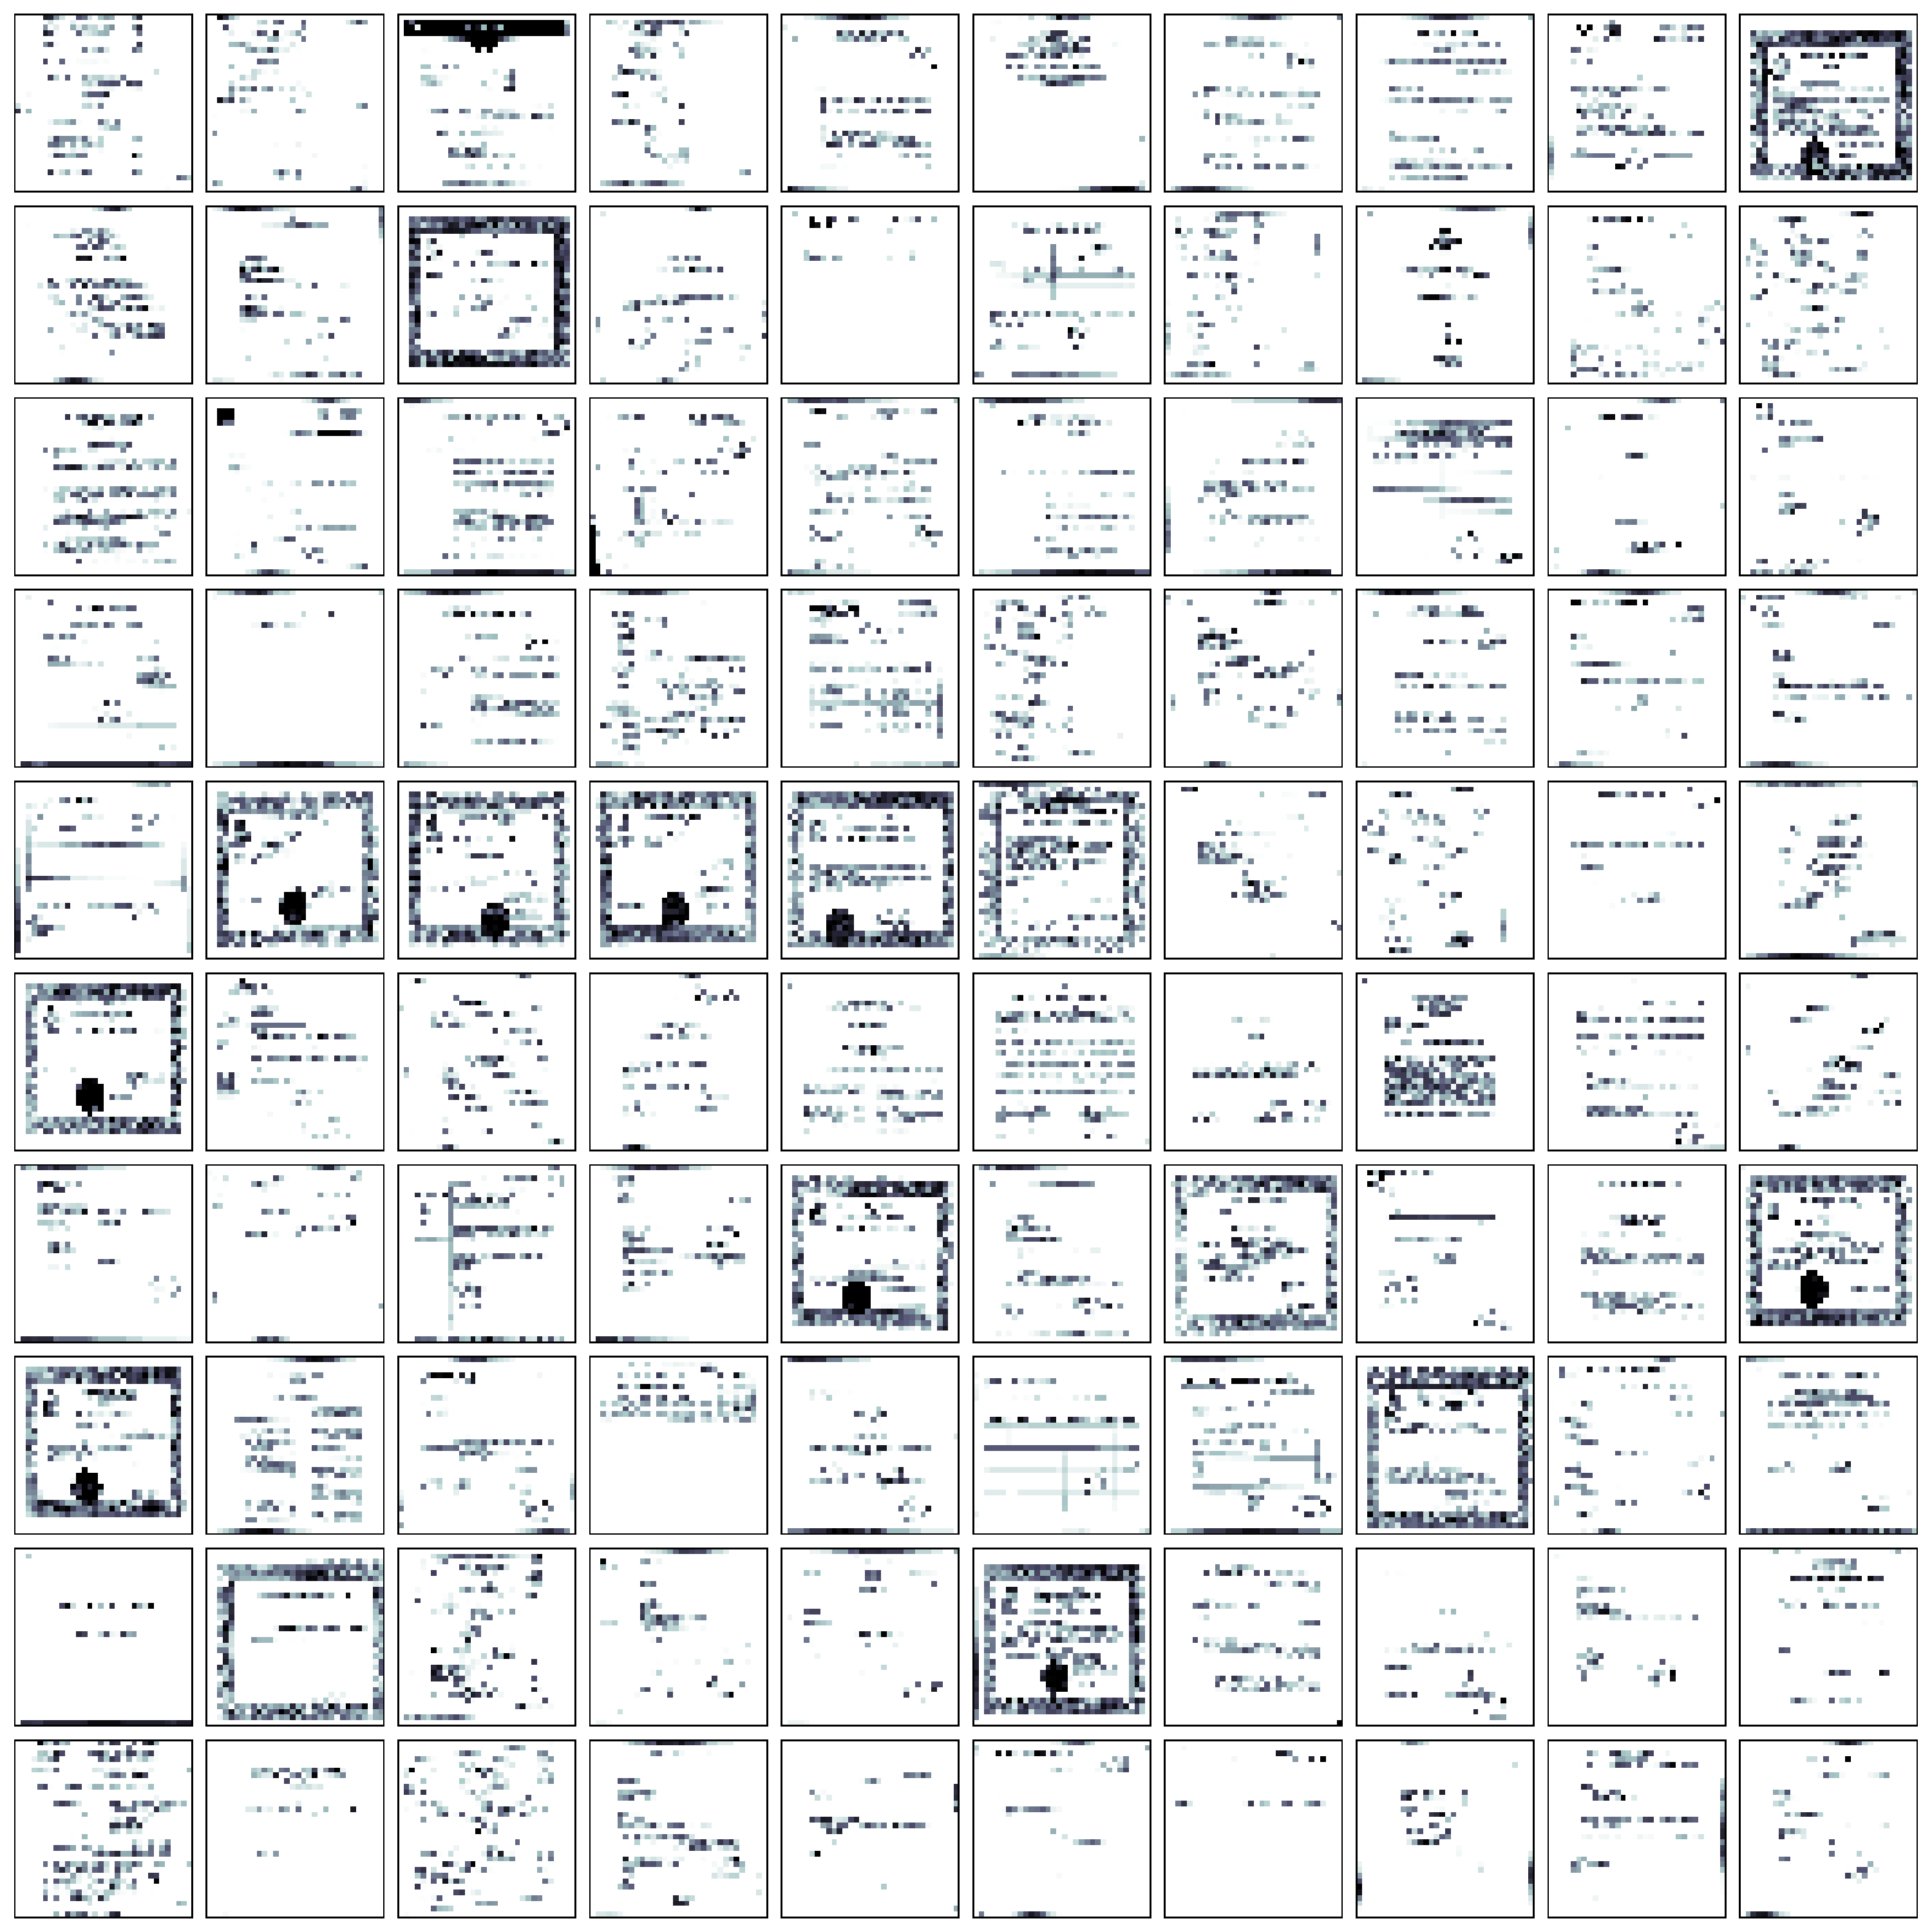
\includegraphics[width=0.5\textwidth]{images/OPTICS/32x32/preprocessed_docs.pdf}
    \caption{The first 100 preprocessed documents of the dataset.
    They were preprocessed in order to have the same characteristics as the images used in \cite{OPTICS1999}.
    The images were preprocessed as discussed in \autoref{pt:32} to 32x32 greyscale pixels, which drastically reduced the quality of the images.
    }
    \label{fig:preprocessed_docs_32x32}
\end{figure}




% OPTIC cluster results
\begin{figure}%
    \centering
    \subfloat[\centering The clusters identified by \ac{optics} of the documents preprocessed according to \autoref{pt:32}.]{{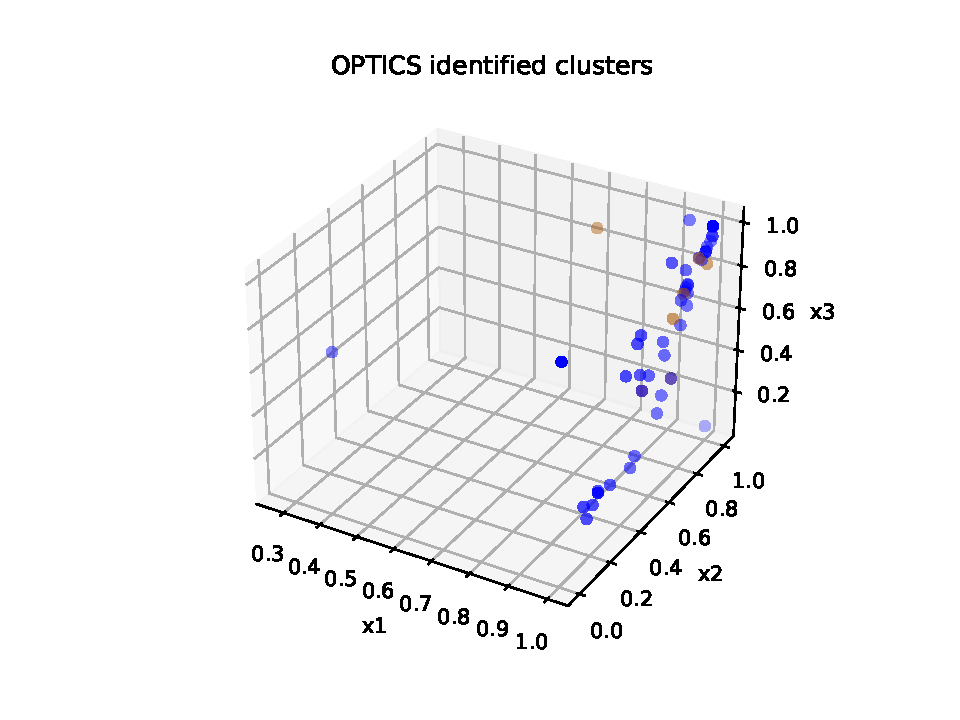
\includegraphics[width=5cm]{images/OPTICS/32x32/OPTICS_cluster_32x32.pdf} }}%
    \qquad
    \subfloat[\centering The clusters identified by \ac{optics} of the documents preprocessed according to \autoref{pt:eigendocs}.]{{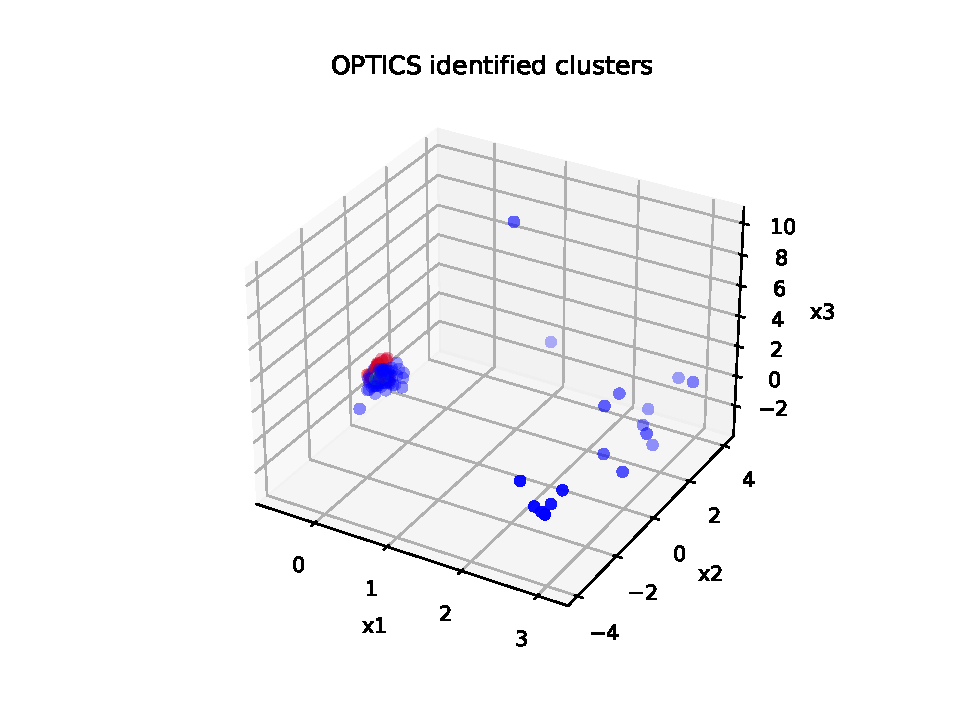
\includegraphics[width=5cm]{images/OPTICS/eigendocs/OPTICS_cluster_eigendocs.pdf} }}%
    \caption{The clusters were extracted from the respective reachability plot in \autoref{fig:reachability_plots}.
    The blue points are noise points, whereas any other colour denotes a cluster.}%
    \label{fig:optics_cluster}%
\end{figure}